\documentclass[12pt,a4paper]{article}

% --- Настройка языка и шрифтов для LuaLaTeX ---
\usepackage{fontspec}
\defaultfontfeatures{Ligatures=TeX,Scale=MatchLowercase}

\setmainfont{Alice-Regular}[
    Path=font/,
    Extension=.ttf,
    BoldFont = Alice-Regular,
    ItalicFont = Alice-Regular,
    BoldItalicFont = Alice-Regular,
    BoldFeatures = {FakeBold=1.6},
    ItalicFeatures = {FakeSlant=0.2},
    BoldItalicFeatures = {FakeBold=1.6,FakeSlant=0.2}
]

\newfontfamily\cyrillicfont{Alice-Regular}[
    Path=font/,
    Extension=.ttf,
    BoldFont = Alice-Regular,
    ItalicFont = Alice-Regular,
    BoldItalicFont = Alice-Regular,
    BoldFeatures = {FakeBold=1.6},
    ItalicFeatures = {FakeSlant=0.2},
    BoldItalicFeatures = {FakeBold=1.6,FakeSlant=0.2}
]

\usepackage{polyglossia}
\setmainlanguage{russian}
\setsansfont{TeX Gyre Heros}
\setmonofont{TeX Gyre Cursor}
\AtBeginDocument{\renewcommand{\textnumero}{{\sffamily №}}}

\usepackage{graphicx}        					% Графика
\usepackage{amsmath, amsfonts, amssymb, amsthm}	% Математика
\usepackage{mathtools}
\usepackage{chemfig}
\usepackage[version=4,arrows=pgf-filled,
            textfontname=sffamily,
            mathfontname=mathsf]{mhchem}
\usepackage[protrusion=false]{microtype}       % Микротипографика
\usepackage{braket} 						% Braket нотация для квантовой механики
\usepackage{unicode-math} 					% Современный пакет для математики в LuaLaTeX
\usepackage{longtable}       				% Таблицы с разрывом страниц
\usepackage{tikz}           				% Рисование
\usepackage[europeanresistors]{circuitikz}	% Рисование электрических схем в европейском стиле
\usepackage{listings}						% Для отображения кода
\usepackage{tabularx}       				% Для таблиц во всю ширину
\usepackage{array}		  					% Для расширенных возможностей таблиц
\usepackage{float}          				% Для точного позиционирования фигур
\usepackage{pgfplots}                          % Для построения графиков
\usepackage{caption}                           % Для настройки подписей к рисункам и таблицам
\usepackage{xfp}                               % Для вычислений в LaTeX
\usepackage{luacode}                           % Для выполнения Lua-кода в документе    
\pgfplotsset{compat=1.18}
\usepackage[paper=letterpaper,
            top=20mm,
            bottom=20mm,
            left=10mm,
            right=10mm,
            footskip=0.4in 
]{geometry}

\usetikzlibrary{arrows.meta}

% --- Колонтитулы ---
\usepackage{fancyhdr}
\pagestyle{fancy}
\fancyhf{}
\setlength{\headheight}{15pt}

% --- Теоремы и окружения ---
\theoremstyle{plain}
\newtheorem{theorem}{Theorem}[section]
\newtheorem{lemma}[theorem]{Lemma}
\newtheorem{proposition}[theorem]{Proposition}
\newtheorem{corollary}[theorem]{Corollary}

\theoremstyle{definition}
\newtheorem{definition}[theorem]{Definition}

\theoremstyle{remark}
\newtheorem{remark}[theorem]{Remark}

\numberwithin{equation}{section}


\renewcommand{\headrulewidth}{0.4pt}
\renewcommand{\footrulewidth}{0.4pt}
\renewcommand\lstlistingname{Листинг}

\lstdefinelanguage{spice}{
	alsoletter={.},
	morecomment=[l]{*},
	morecomment=[l]{;},
	morekeywords={.DC, .dc, .TRAN, .tran, .AC, .ac, .OP, .op, .SAVE, .save, .PROBE, .probe, .END, .end, .PARAM, .param, .MODEL, .model, .SUBCKT, .subckt, .ENDS, .ends, .INCLUDE, .include, .LIB, .lib, .IC, .ic, .NODESET, .nodeset, .STEP, .step, .PRINT, .print, .PLOT, .plot},
	sensitive=false
}

\lstdefinestyle{main}{
	backgroundcolor=\color{gray!8},   
	commentstyle=\color{green!50!black}\itshape,
	keywordstyle=\color{blue!80!black}\bfseries,
	numberstyle=\small\color{darkgray},
	stringstyle=\rmfamily\color{orange!90!black},
	basicstyle=\ttfamily\small,
	breakatwhitespace=false,         
	breaklines=true,                   
	keepspaces=true,                 
	numbers=left,                    
	numbersep=8pt,                  
	showspaces=false,                
	showstringspaces=false,
	showtabs=false,                  
	tabsize=4,
	frame=single,
	framerule=0.5pt,
	rulecolor=\color{gray!30},
	captionpos=t
}	

\lstset{style=main}

\newcolumntype{C}{>{\centering\arraybackslash}X}
\renewcommand{\arraystretch}{1.25}

\begin{luacode*}
    data = require("data")
    include = require("include")
    handle = require("handle")
\end{luacode*}

\newcommand{\VariantN}{1}
\newcommand{\LabNumber}{1}
\newcommand{\LabTitle}{Входной язык симулятора SPICE}
\newcommand{\Discipline}{Разработка САПР}

\title{
	Министерство науки и высшего образования 
    
    Российской Федерации
    
    Национальный исследовательский университет «МИЭТ»
    
    Институт интегральной электроники имени академика 
    
    К. А. Валиева

	\vspace{2em}
}
\author{
}
\date{}

\begin{document}

\maketitle
\thispagestyle{fancy}

\begin{center}
\Large Отчёт по Лабораторной работе \textnumero~\LabNumber\\
по дисциплине «\Discipline»\\
«\LabTitle»
\end{center}

\vspace{15em}

\begin{flushright}
	Выполнил студент группы ЭН-$35$\\
	Андреев И. А.\\
    Вариант \textnumero~\VariantN\\
	Проверил преподаватель института ИнЭл\\
    Щучкин Евгений Юрьевич
\end{flushright}

\cfoot{Москва 2026}

\pagebreak

\fancyhead[L]{\LabTitle}
\fancyhead[R]{\Discipline}
\fancyfoot[C]{\thepage}

\fancyhead[L]{Теория}
\fancyhead[R]{\LabTitle}

\begin{center}
\Large\textbf{Лабораторная работа $\LabNumber$}
\end{center}

\textbf{Цель работы:} получить навыки описания электрических схем и заданий на 
моделипрования на входном языке симулятора \textbf{SPICE}, выполнить статический 
анализ (\textrm{.DC}) и динамический анализ (\textrm{.TRAN}) в САПР Symica DE.

\begin{center}
\LARGE\textbf{\LabTitle}
\end{center}

\section{Пример 1. Ток через резистор (статический анализ \textrm{.DC}) }

Схема приведена на рисунке $\ref{fig:task1_curcuit}$, её SPICE-описание — 
в листинге $\ref{lst:task1}$, результат моделирования — на рисунке 
$\ref{fig:task1_plot}$.

\begin{figure}[H]
    \centering
    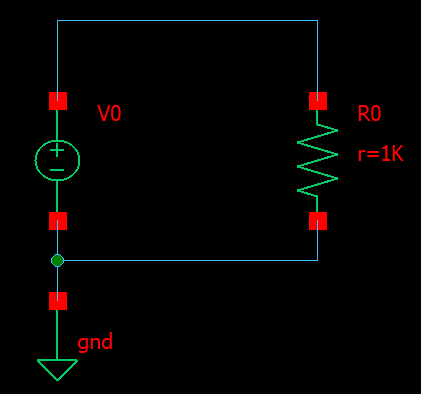
\includegraphics[width=0.5\textwidth]{image/task1_curcuit.png}
    \caption{Схема: источник $V_0$ и резистор $R_0$ (1кОм) между узлами 1 и gnd.}
    \label{fig:task1_curcuit}
\end{figure}

\begin{lstlisting}[language=spice,caption={SPICE-описание схемы примера 1},label={lst:task1}]
* Resistor current

V0 1 gnd 5
R0 1 gnd 1k

.DC V0 0 5 0.1
.PROBE I(R0)
.END
\end{lstlisting}

\begin{figure}[H]
    \centering
    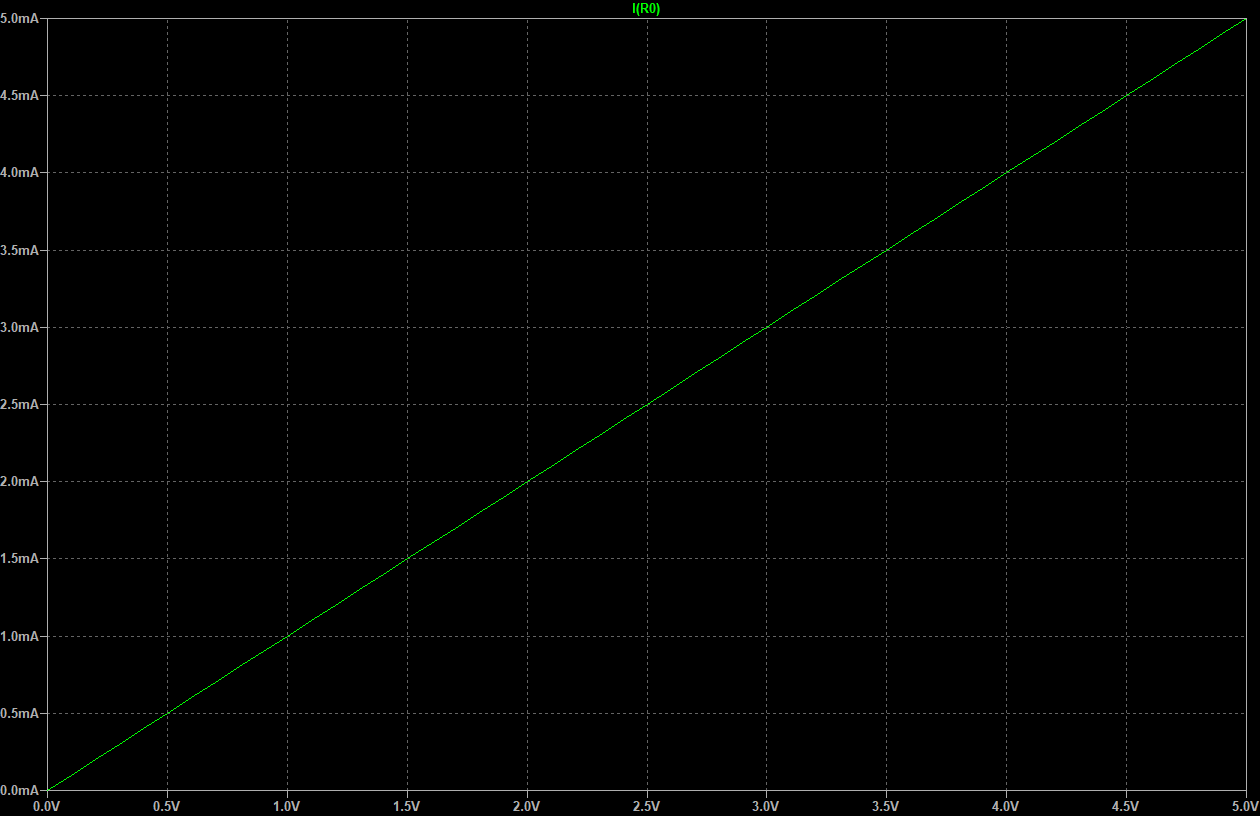
\includegraphics[width=\textwidth]{image/task1_plot.png}
    \caption{Зависимость тока через резистор $R_0$ от напряжения источника $V_0$.}
    \label{fig:task1_plot}
\end{figure}

\textbf{Результат:} график — прямая из начала координат в точку $5$ мА при $5$ В.

\section{Пример 2. RC-цепь (динамический анализ \textrm{.TRAN}) }

Схема приведена на рисунке $\ref{fig:task2_curcuit}$, её SPICE-описание — в 
листинге $\ref{lst:task2}$, результат моделирования — на рисунке 
$\ref{fig:task2_plot}$.

\begin{figure}[H]
    \centering
    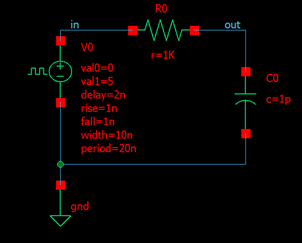
\includegraphics[width=0.5\textwidth]{image/task2_curcuit.png}
    \caption{Импульсный источник напряжения, подключенный к интегрирующей RC-цепи.}
    \label{fig:task2_curcuit}
\end{figure}

\begin{lstlisting}[language=spice,caption={SPICE-описание схемы примера 2},label={lst:task2}]
*RC-net

V0 in 0 PULSE(0 5 2n 1n 1n 10n 20n)
R0 in out 1K
C0 out 0 1p

.TRAN 1n 100n
.SAVE V(in) V(out)
.END
\end{lstlisting}

\begin{figure}[H]
    \centering
    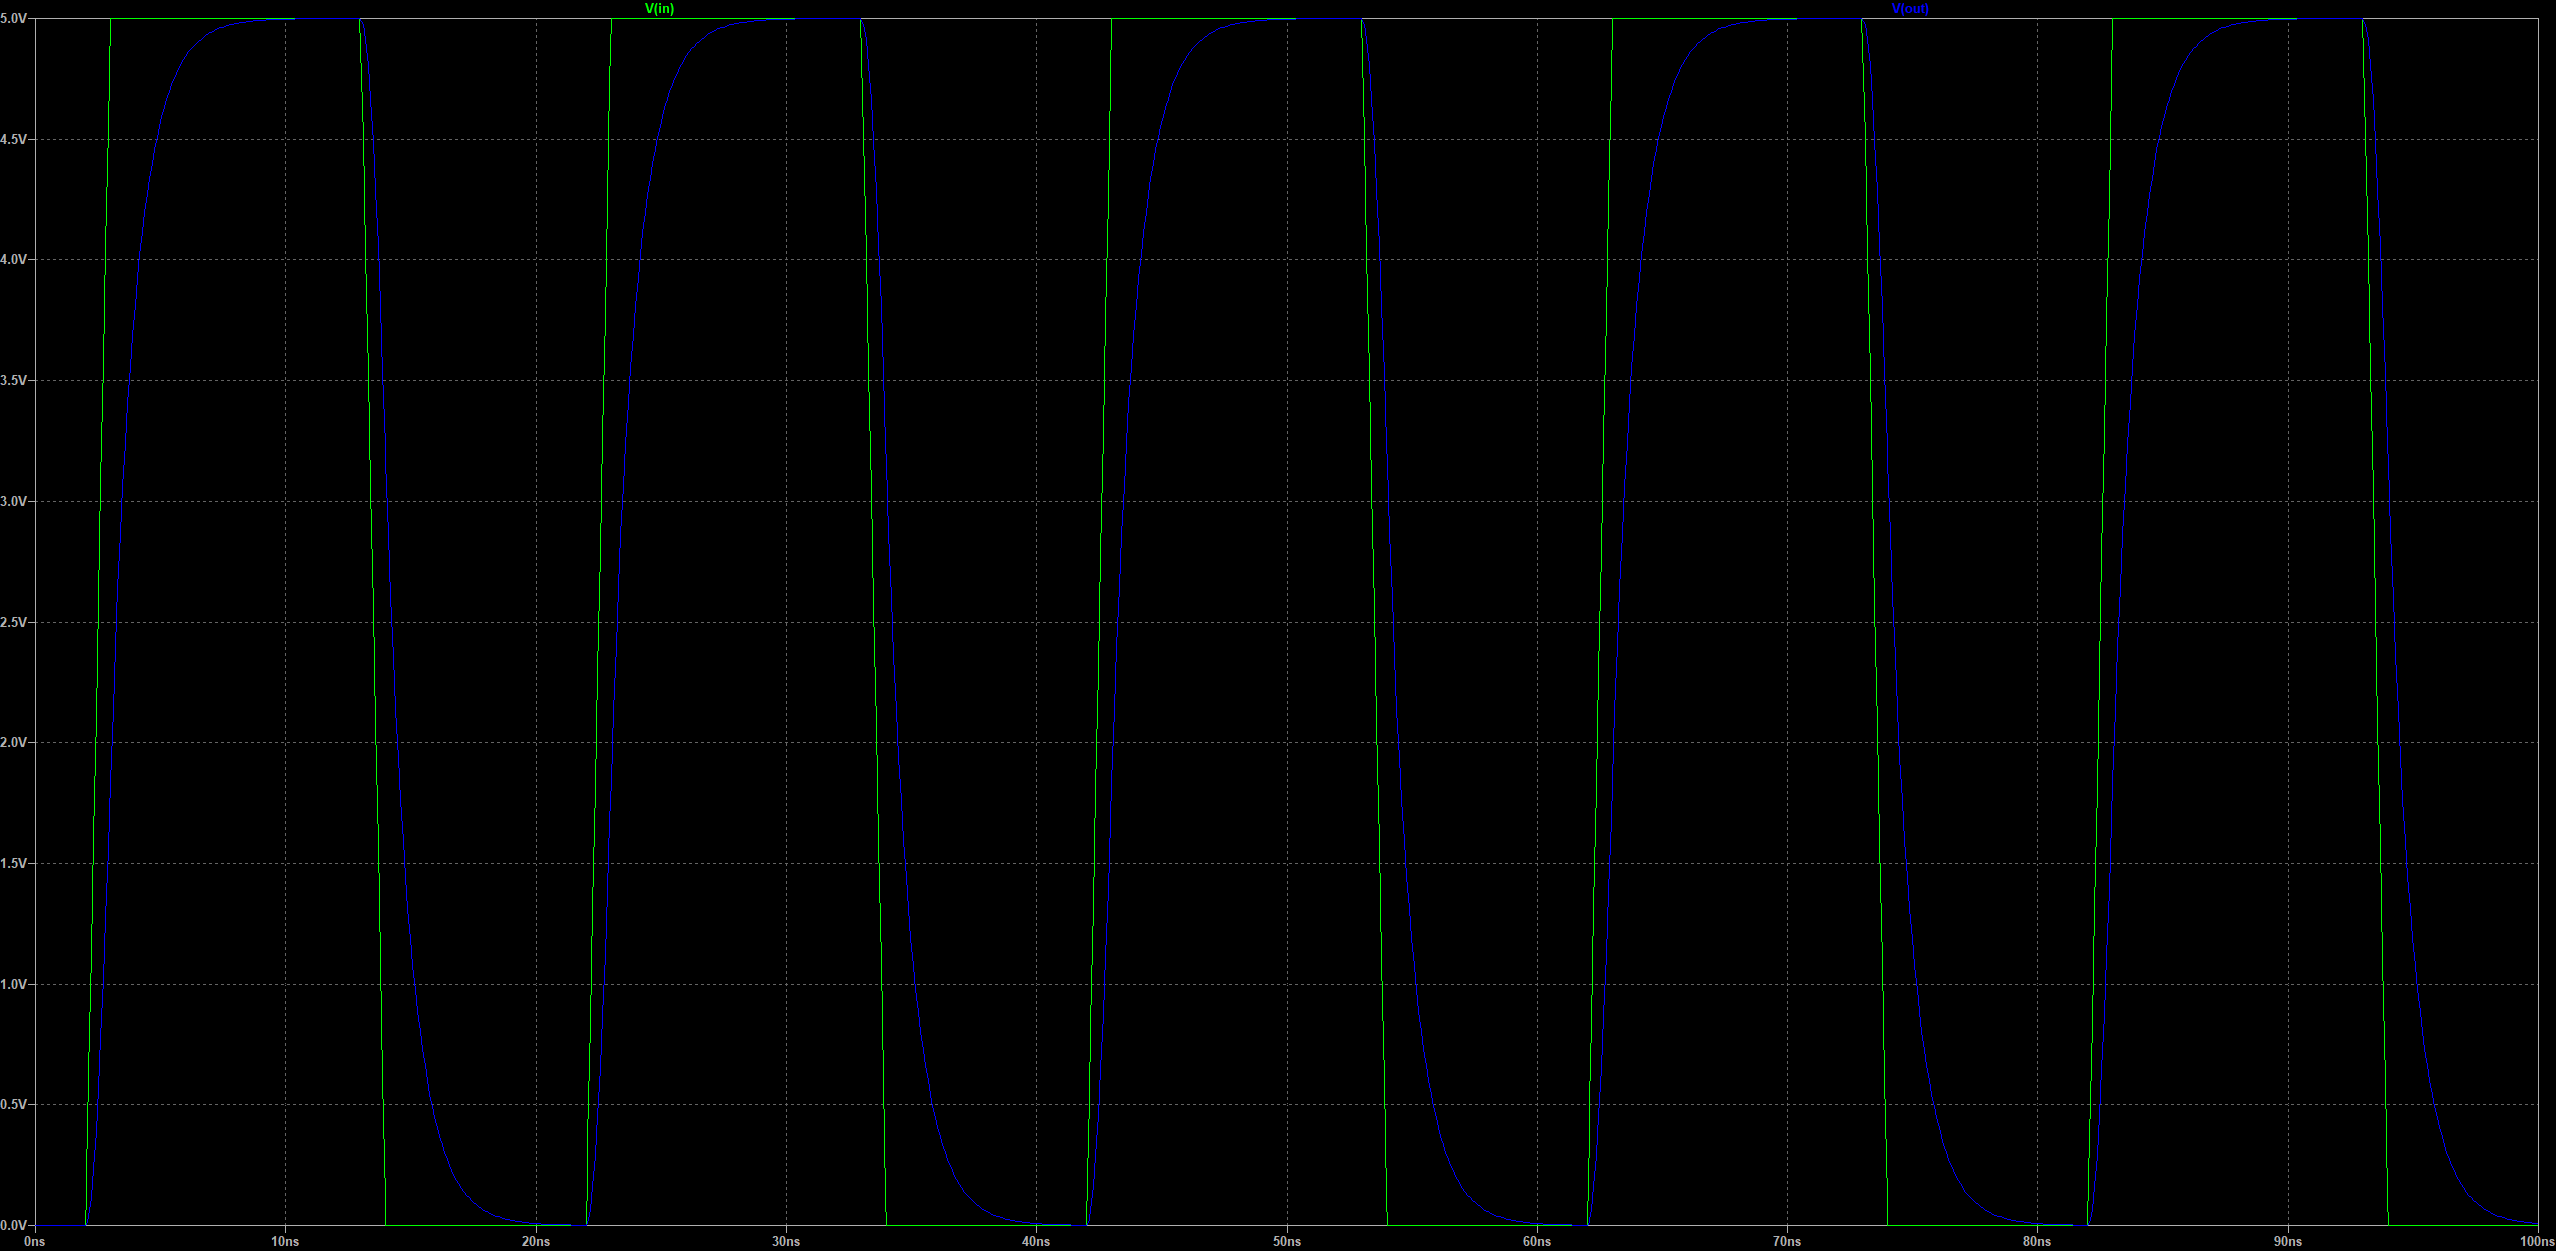
\includegraphics[width=\textwidth]{image/task2_plot.png}
    \caption{Напряжения на входе (in) и выходе (out) интегрирующей RC-цепи.}
    \label{fig:task2_plot}
\end{figure}

\textbf{Результат:} график — сглаженный импульсный сигнал с заваленными фронтами.

\section{Пример 3. Подсхемы (\textrm{.SUBCKT}) }

Схема приведена на рисунке $\ref{fig:task3_curcuit}$, её SPICE-описание — в
листинге $\ref{lst:task3}$, результат моделирования — на рисунке 
$\ref{fig:task3_plot}$.

\begin{figure}[H]
    \centering
    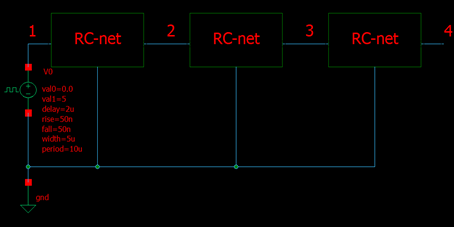
\includegraphics[width=0.5\textwidth]{image/task3_curcuit.png}
    \caption{Схема из трёх одинаковых RC-звеньев, описанных подсхемой.}
    \label{fig:task3_curcuit}
\end{figure}

\begin{lstlisting}[language=spice,caption={SPICE-описание схемы примера 3 с подсхемой},label={lst:task3}]
* Subcircuit example

* 1. Описание подсхемы rc_net
.SUBCKT rc_net in out
R1 in out 1k
C1 out 0 10p
.ENDS rc_net

* 2. Основная схема
V0 1 0 PULSE(0 5 2u 50n 50n 5u 10u)
X1 1 2 rc_net
X2 2 3 rc_net
X3 3 4 rc_net

.TRAN 10n 20u
.END
\end{lstlisting}

\begin{figure}[H]
    \centering
    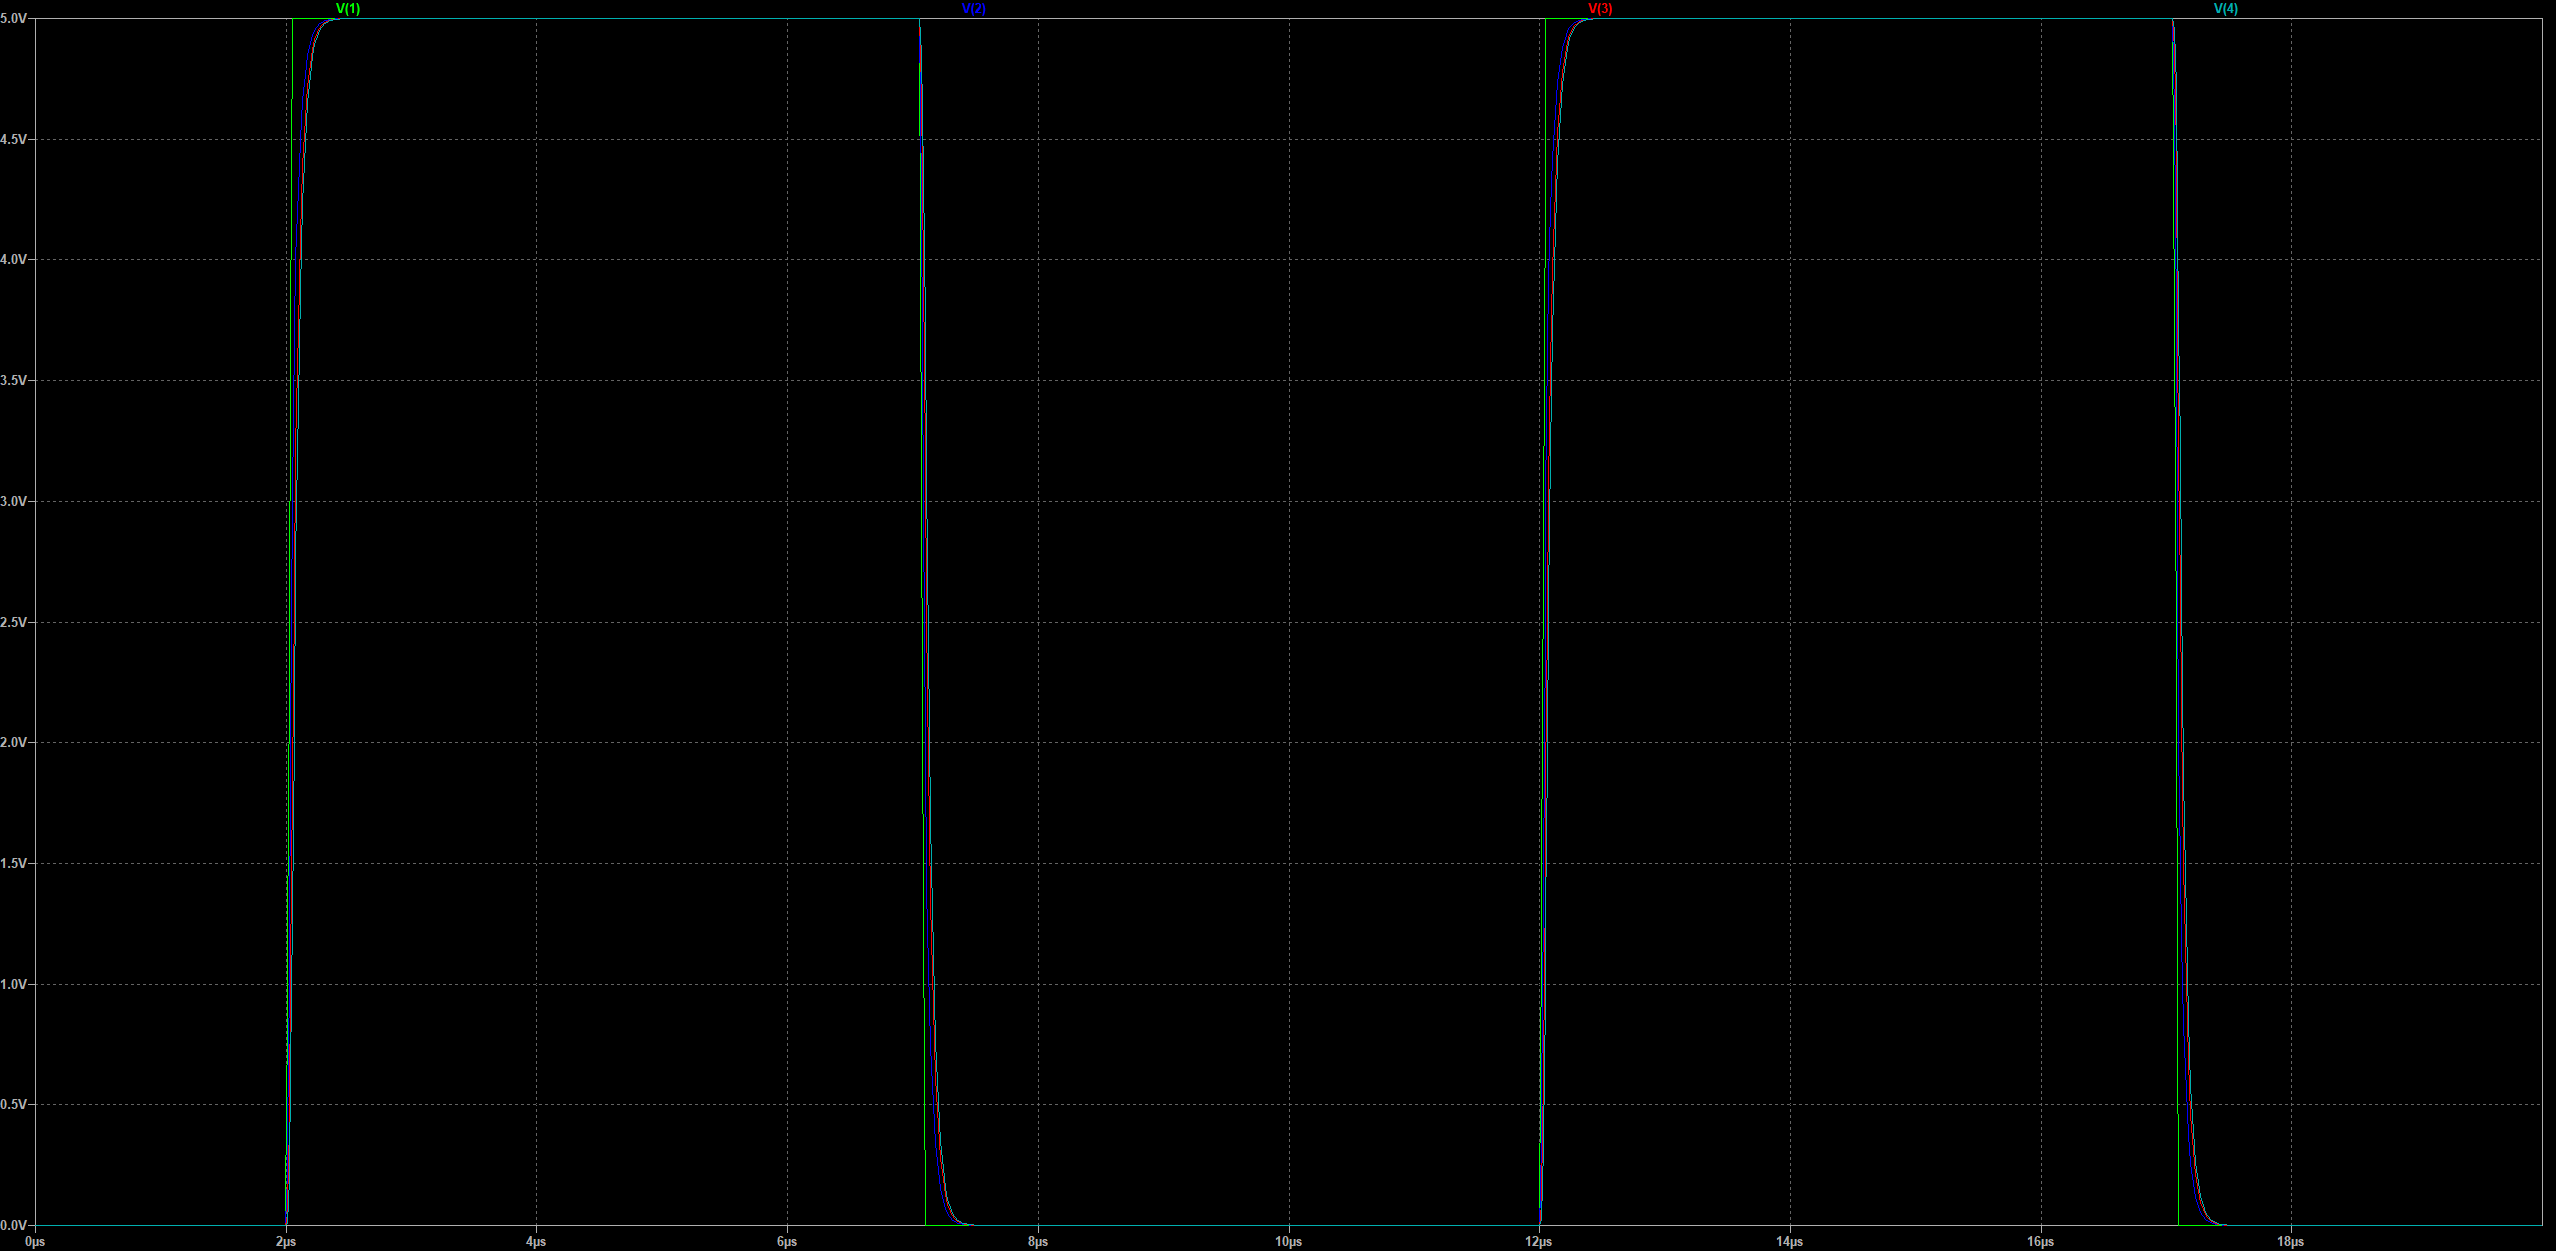
\includegraphics[width=\textwidth]{image/task3_plot.png}
    \caption{Напряжения в узлах $1 \dots 4$ схемы из трёх RC-звеньев.}
    \label{fig:task3_plot}
\end{figure}

\textbf{Результат:} график — представляет из себя $1$ сигнал в форме импульса, 
и $3$ сглаженных его версии, видно, что каждый последующий сигнал имеет более
сглаженный вид, чем предыдущий.

\section{Задание 1. Резистивный делитель (статический анализ) }

Схема делителя приведена на рисунке $\ref{fig:task4_curcuit}$. Номиналы 
резисторов рассчитаны так, чтобы при $V_\text{in} = 5$ В напряжение в средней
точке равнялось значению $V_\text{out} = 1$ В. Расчёт и результаты моделирования
приведены в таблице $\ref{tab:task4}$.

\vspace{1em}

\noindent\begin{tabularx}{\textwidth}{|C|C|C|C|}
    \hline
    $V_\text{out} = 1$ В & $R_0$, кОм & $R_1$, кОм & $V_\text{out} = 1$ при $V_\text{in} = 5$, В \\
    \hline
\end{tabularx}

\begin{figure}[H]
    \centering
    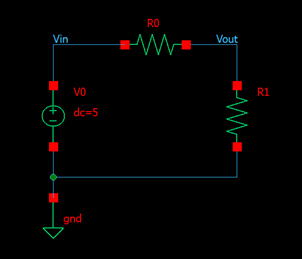
\includegraphics[width=0.5\textwidth]{image/task4_curcuit.png}
    \caption{Принципиальная схема резистивного делителя напряжения.}
    \label{fig:task4_curcuit}
\end{figure}

\end{document}